% ============================================
% 6 问题3：未知类别鉴别
% ============================================
\section{问题3：未知类别鉴别}

\subsection{研究方法}

采用\textbf{四法共识策略}，以未风化已知样品为训练集，对 8 个未知样品进行分类：

\begin{enumerate}[label=(\arabic*)]
    \item \textbf{BaO 规则}：$\text{BaO} > 3.14\% \rightarrow$ 铅钡玻璃
    \item \textbf{PbO 规则}：$\text{PbO} > 5.46\% \rightarrow$ 铅钡玻璃
    \item \textbf{决策树}：以 $\text{BaO} \leq 3.14\%$ 为分类边界
    \item \textbf{LDA}：多变量线性判别
\end{enumerate}

四种方法独立投票，以多数票（$\geq 2/4$）确定最终类别，全票（4/4）为高置信度分类。

\subsection{分类结果}

\begin{table}[H]
    \centering
    \caption{8 个未知样品的四法分类结果}
    \label{tab:classification}
    \begin{tabular}{c c c c c c c c c}
        \toprule
        \textbf{样品} & \textbf{风化} & \textbf{$\text{SiO}_2$} & \textbf{$\text{K}_2\text{O}$} & \textbf{PbO} & \textbf{BaO} & \textbf{共识} & \textbf{票数} & \textbf{置信度} \\
        \midrule
        A1 & 无 & 78.5 & 0 & 0 & 0 & \textbf{高钾} & 4/4 & 高 \\
        A2 & 风化 & 37.8 & 0 & 34.3 & 0 & \textbf{高钾} & 3/4 & 中 \\
        A3 & 无 & 32.0 & 1.4 & 39.6 & 4.7 & \textbf{铅钡} & 4/4 & 高 \\
        A4 & 无 & 35.5 & 0.8 & 24.3 & 8.3 & \textbf{铅钡} & 4/4 & 高 \\
        A5 & 风化 & 64.3 & 0.4 & 12.2 & 2.2 & \textbf{高钾} & 3/4 & 中 \\
        A6 & 风化 & 93.2 & 1.4 & 0 & 0 & \textbf{高钾} & 4/4 & 高 \\
        A7 & 风化 & 90.8 & 1.0 & 0 & 0 & \textbf{高钾} & 4/4 & 高 \\
        A8 & 无 & 51.1 & 0.2 & 21.2 & 11.3 & \textbf{铅钡} & 3/4 & 中 \\
        \bottomrule
    \end{tabular}
\end{table}

最终判定：
\begin{itemize}
    \item \textbf{高钾玻璃}：A1、A2、A5、A6、A7
    \item \textbf{铅钡玻璃}：A3、A4、A8
\end{itemize}

\subsection{异常样品分析}

\textbf{A2}（风化，$\text{PbO} = 34.3\%$，$\text{BaO} = 0$）是最值得关注的异常：
\begin{itemize}
    \item PbO 含量极高（$> 30\%$），具有铅钡玻璃的典型特征
    \item 但 BaO 完全未检出——而训练集中所有铅钡玻璃 $\text{BaO} > 3.4\%$
    \item 可能解释：（1）纯铅玻璃（不含钡的独立类型）；（2）极端风化导致 BaO 完全流失（但 BaO 通常稳定）
    \item 建议标记为"待确认"，可能是第三种玻璃类型
\end{itemize}

\textbf{A5}（风化，$\text{PbO} = 12.2\%$，$\text{BaO} = 2.2\%$）：
\begin{itemize}
    \item PbO 中等但 BaO 低于 $3.14\%$ 阈值
    \item 风化校正后 $\text{BaO} = 2.76\%$，仍低于阈值
    \item 更可能是风化高钾玻璃含少量铅杂质
\end{itemize}

\subsection{敏感性分析}

\textbf{阈值扰动}：BaO 阈值在 $\pm 20\%$（$2.51\%\sim3.77\%$）范围内扰动，\textbf{0/8 样品分类变化}。A5（$\text{BaO} = 2.16\%$）即使阈值降至 $2.51\%$ 也不会越界。

\textbf{风化校正验证}：对 4 个风化未知样品分别用铅钡和高钾校正向量修正后重分类——所有样品分类不变。

\textbf{多方法一致性}：

\begin{table}[H]
    \centering
    \caption{四种分类方法的一致性矩阵}
    \label{tab:consensus}
    \begin{tabular}{l c c c c}
        \toprule
        & \textbf{BaO 规则} & \textbf{PbO 规则} & \textbf{决策树} & \textbf{LDA} \\
        \midrule
        BaO 规则 & 8 & 6 & 8 & 7 \\
        PbO 规则 & —— & 8 & 6 & 5 \\
        决策树 & —— & —— & 8 & 7 \\
        \bottomrule
    \end{tabular}
\end{table}

BaO 规则与决策树完全一致（8/8），PbO 规则与 LDA 分歧最大（5/8）。

\subsection{结论}

\begin{enumerate}[label=(\arabic*)]
    \item BaO 规则是最稳健的分类方法，对风化和阈值扰动均不敏感
    \item 分类结果对测量误差和阈值选择高度鲁棒
    \item A2 值得进一步研究，可能代表铅钡玻璃之外的第三种类型
\end{enumerate}

\begin{figure}[H]
    \centering
    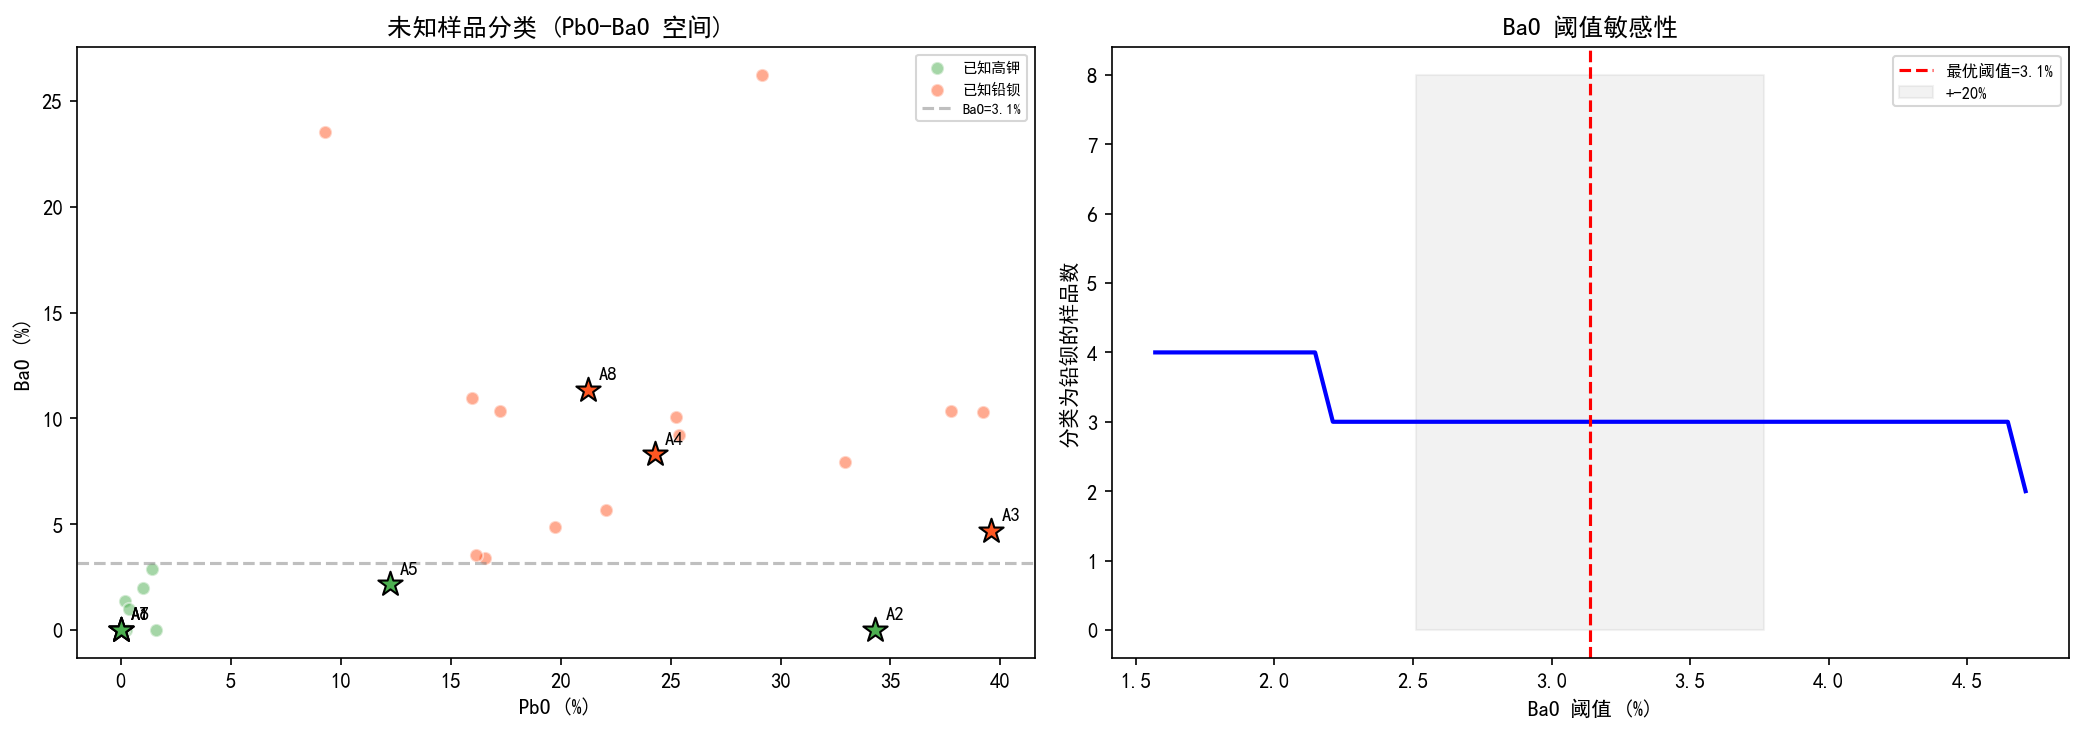
\includegraphics[width=0.85\textwidth]{../analysis/fig3_classification.png}
    \caption{未知样品分类图（PbO-BaO 散点 $+$ 阈值敏感性曲线）}
    \label{fig:classification_fig}
\end{figure}
